\documentclass{X:/Documents/Coding/Latex/myassignment}
\title{Mathematical Biology Assignment 3 \& 4}

\begin{document}
\maketitle
Normally I would paraphrase the  the questions, but instead I have appended the question sheet to the end
\section{Assignment 3}
\begin{enumerate}
	\item to break down the problem into pieces:
	\begin{itemize}
		\item The cells $(c,m,n)$ all proliferate logistically ($c$ greater rate than $n$).
		\item $m$ increases (and saturates) with $a$
		\item $c,n,m$ all move by random motion, and $m$ moves via chemotaxis with gradient of $a$
		\item $a$ is produced constantly by $c$ and decays `naturally'
		\item $m$ kills $c$ at a rate proportional to $a$ concentration. 
		\item $a$ moves via diffusion
	\end{itemize}
	Constants:
	\begin{itemize}
		\item Proliferation rates of $c,m,n$ respectively $p_c,p_m,p_n$ with $p_c > p_n$
		\item Carrying capacities for the cells $k_c,k_m,k_n$
		\item $l_a$ describes the early growth rate of $m$ with respect to $a$
		\item $\beta_m$ is the death rate of cancer cells due to macrophages and $\beta_a$ is the decomposition of MCP
		\item $\chi$ is the chemotactic constant for the macrophages
	\end{itemize}
	\begin{align*}
		\dd ct &= \nabla \left(D_c \nabla c\right) + p_c c(1 - \frac{c}{k_c}) - \beta_m m c\\
		\dd nt &= \nabla \left(D_n \nabla n\right) + p_n n(1 - \frac{n}{k_n})\\
		\dd mt &= \nabla \left(D_m \nabla m\right) - \chi \nabla \left[m \nabla a\right] + \frac{p_m a}{l_a+a} m(1 - \frac{m}{k_m})\\
		\dd at &= \nabla \left(D_a \nabla a\right) + p_a c - \beta_a\\
	\end{align*}
	Where since this is for $1D$ $\nabla := \odd{}x$
	%not sure about the chi term





	%q2
	\item 
	\begin{enumerate}
		\item I'm going to let $(\tilde{b}, \tilde{p}) := \epsilon(b_1,p_1)e^{iqx+\lambda t}$ 
		\begin{align*}
			\dd bt &= \mu \ddn bx2 + \frac{\gamma b}{1+ b} - \frac{b p }{\kappa + b}\\
			\lambda \tilde{b} &= -q^2 \mu \tilde{b} + \frac{\gamma \tilde{b}}{1 + \tilde{b}} - \frac{\tilde{b} (1 + \tilde{p})}{\kappa + b}\\
			\lambda &= -q^2 \mu + \frac{\gamma}{1 + \tilde{b}} - \frac{(1+\tilde{p})}{\kappa + \tilde{b}}\\
		\end{align*}
		To leading order, $(\tilde{b},\tilde{p})$ is negligible (assuming $\epsilon \ll 1$) this gives
		\[\lambda = -q^2 \mu + \gamma - \frac{p}{\kappa}\]
		For the $p$ equation:

		\begin{align*}
			\dd pt &= \ddn px2 - \delta \dd{}x \left(p \dd bx\right) + \alpha (1 + \sigma b -p)\\
			\dd pt &= \ddn px2 - \delta \left(\dd px \dd bx + p \ddn bx2\right) + \alpha (1 + \sigma b -p)\\
			\lambda \tilde{p} &= -q^2 \tilde{p} - \delta\left(-q ^2\tilde p \tilde b - (1+ \tilde{p})q^2 \tilde{b}\right)+ \alpha (1 + \sigma \tilde{b} - (1 + \tilde{p}))\\
			\lambda \tilde{p} &= -q^2 \tilde{p} - \delta\left(-2q ^2\tilde p \tilde b - q^2 \tilde{b}\right)+ \alpha (\sigma \tilde{b} - \tilde{p}))\\
			\lambda  &= -q^2 - \delta\left(-2q ^2 \tilde b - q^2 \frac{\tilde{b}}{\tilde{p}}\right)+ \alpha (\sigma \frac{\tilde{b}}{\tilde{p}} - 1))\\
			% \lambda &= -q^2 - \delta\left(-q ^2\tilde b - q^2 \tilde{b} - q^2\frac{b_1}{p_1}\right)+ \alpha (\sigma \frac{b_1}{p_1} - 1)\\
			% \lambda &= -q^2 - \alpha + \frac{b_1}{p_1}\left(- q^2 + \alpha \sigma \right)
		\end{align*}
		At order $\bigo(\epsilon)$
		\begin{align*}
			\lambda \tilde{p} &= -q^2 \tilde{p} - \delta\left(-q^2 \tilde{b}\right)+ \alpha (\sigma \tilde{b} - \tilde{p})\\
			\lambda &= -q^2 - \delta\left(-q^2 \frac{b_1}{p_1}\right)+ \alpha (\sigma \frac{b_1}{p_1} - 1)\\
			\lambda &= -q^2  - \alpha - \frac{b_1}{p_1}\left( -q^2 \delta+ \alpha \sigma \right)\\
		\end{align*}
		Either $\frac{b_1}{p_1} = 0$ or $q^2 \delta = \alpha \sigma $ for the answer required...
		%not done yet

		%need to end up with
		%\[\lambda = -q^2 - \alpha\]
		\item Instabilities occur for lambda with positive real part. So, the most likely instabilities will occur for values of $q$ which give the largest $\lambda$. Hence in this case, the smallest values of $q$ will give the most likely instabilities. I.e. the wavenumbers with highest frequency 
		\item I am going to drop the bars for simplicity sake, I.e. $(b,1+\sigma b)$

		Existence :
		\begin{align*}
			\dd bt &= \mu \ddn bx2 + \frac{\gamma b}{1+ b} - \frac{b p }{\kappa + b}\\
			0 &= \frac{\gamma b}{1+ b} - \frac{b(1+ \sigma b)}{\kappa + b}\\
			0 &= \gamma(\kappa + b)  - (1+b)(1+ \sigma b)\\
			0 &= \gamma \kappa +\gamma b  - 1 - b - \sigma b - \sigma b^2 \\
		\end{align*}
		%^^^^something wrong here

		\begin{align*}
			\dd pt &= \ddn px2 - \delta \dd{}x \left(p \dd bx\right) + \alpha (1 + \sigma b -p)\\
			 &= \alpha (1 + \sigma b -(1 + \sigma b))\\
			 &= (1 -1 +\sigma b - \sigma b) = 0
		\end{align*}
		Stability:
		\[(b, p) = (\bar b, 1 + \sigma \bar b) + \epsilon (\bar b_1, \bar p_1) e^{iqx + \lambda t}\]
		I will call the perturbation part $(\hat b, \hat p)$
		\begin{align*}
			\dd bt &= \mu \ddn bx2 + \frac{\gamma b}{1+ b} - \frac{b p }{\kappa + b}\\
			\lambda \hat b &= -\mu q^2 \hat b + \frac{\gamma (\bar b + \hat b)}{1+ (\bar b + \hat b)} - \frac{(\bar b + \hat b)(1 + \sigma \bar b + \hat p) }{\kappa + (\bar b + \hat b)}\\
		\end{align*}

		\begin{align*}
			\dd pt &=  \ddn px2 - \delta \dd{}x \left(p \dd bx\right) + \alpha (1 + \sigma b -p)\\
			\lambda \hat p &= -q^2 \hat p - \delta \left(-q^2\hat{b}\hat{p}  - q^2 \hat{b}(1 + \sigma\bar{b} + \hat{p})\right) + \alpha (1 + \sigma (\bar{b} + \hat{b}) -(1 + \sigma \bar{b} +\hat{p}))
		\end{align*}
		This state will be linearly stable if both of these $\lambda$ equations give  $\lambda < 0$

		\begin{align*}
			\lambda = \frac{1}{\hat{b}} \left( -\mu q^2 \hat b + \frac{\gamma (\bar b + \hat b)}{1+ (\bar b + \hat b)} - \frac{(\bar b + \hat b)(1 + \sigma \bar b + \hat p) }{\kappa + (\bar b + \hat b)}\right) &< 0\\
			 -\mu q^2 \hat b + \frac{\gamma (\bar b + \hat b)}{1+ (\bar b + \hat b)} - \frac{(\bar b + \hat b)(1 + \sigma \bar b + \hat p) }{\kappa + (\bar b + \hat b)} &< 0\\
		\end{align*}

		\begin{align*}
			\lambda = \frac{1}{\hat{p}}\left(-q^2 \hat p - \delta \left(-q^2\hat{b}\hat{p}  - q^2 \hat{b}(1 + \sigma\bar{b} + \hat{p})\right) + \alpha (1 + \sigma (\bar{b} + \hat{b}) -(1 + \sigma \bar{b} +\hat{p}))\right) < 0
		\end{align*}

		Need to get
		\begin{align*}
			\frac{\gamma}{(1 + \bar{b})^2} - \frac{\kappa(1 + \sigma b)}{(\kappa + \bar{b})^2} - \alpha - (1 + \mu)q^2 < 0\\
			\frac{\alpha \kappa (1 + \sigma \bar{b})}{(\kappa + \bar{b})^2} - \frac{\alpha \gamma}{(1 + \bar{b})^2} + \frac{\alpha \sigma \bar{b}}{\kappa + \bar{b}} + \left(\mu q^2 +  \mu \alpha + \delta (1+ \sigma \bar{b}) G(\bar{b}) - F(\bar{b})\right) q^2 > 0
		\end{align*}
		Where
		\[F(\bar{b}) = \frac{\bar{b}(1 + \sigma \bar{b})(1 - \kappa)}{(1 + \bar{b})(\kappa + \bar{b})^2}, \quad G(\bar b) = \frac{\bar{b}}{\kappa + \bar b}\]
		%He wrote k at the end instead of kappa?
		%not done yet
	\end{enumerate}
	\item 
	\begin{enumerate}
		\item The $\chi$ terms represent chemotaxis along a gradient. Since negative coefficients correspond to moving up a gradient (towards higher concentrations), $c_1$ is the $\beta$-amyloid, and $c_2$ is the TNF-$\alpha$.
		\item Sub in $(m_0,c_{10},c_{20})$. The first equation is trivially zero.
		% \begin{align*}
		% 	\dd mt &= D_m \ddn mx2 - \chi_1 \dd{}x \left(m \dd {c_1} x\right) + \chi_2 \dd{}x \left(m \dd{c_2}x\right)\\
		% \end{align*}
		\begin{align*}
			\dd{c_1} t &= D_1 \ddn{c_1}x2 + a_1 m - b_1 c_1\\
			0 &= 0 + a_1m_0 - b_1 c_{10}\\
			c_{10} &= \frac{a_1 m_0}{b_1}
		\end{align*}
		\begin{align*}
			\dd{c_2} t &= D_2 \ddn{c_2}x2 + a_2 m - b_2c_2\\
			0 &= 0 + a_2 m_0 - b_2 c_{20}\\
			c_{20} &= \frac{a_2 m_0}{b_2}
		\end{align*}
		\item $\epsilon_1 = \frac{D_m}{D_1}$. This is the ratio of the rates of diffusion of glial cells and $\beta$-amyloid. Similarly, $\epsilon_2$ is the ratio of the rates of diffusion of glial cells and TNF-$\alpha$.
		Setting these simultaneously to zero corresponds to $D_m \ll D_1,D_2$. I.e. that the rate of diffusion of glial cells is significantly lower than that of the protein and chemical. Explicitly setting these to zero is by either letting $D_m = 0$ or both $D_1,D_2 \to \infty$. I.e. by assuming glial cells do not diffuse or that the protein and chemical both diffuse instantly.
		\item Assume $(m,c_1,c_2) = (1,1,1)$. Linear stability analysis - using the fact that $\dd mx = \dd{c_1}x = \dd{c_2} x = 0$ for $x=0,l$ (under the changed system):
		\[(m,c_1,c_2) = \vec 1 + \epsilon (m_1,c_{11},c_{21}) \cos(qx)e^{\omega t}\]

		Since we are setting $\epsilon_1 = \epsilon_2 = 0$ we only need to consider the first equation
		\begin{align*}
			\dd mt &= \ddn mx2 - A_1 \dd{}{x} \left(m \dd{c_1}{x}\right) + A_2 \dd{}x \left(m \dd{c_2}{x}\right)\\
			\omega \bar{m} &= -q^2 \bar{m} - A_1 \left(-q^2 \bar{c_1}(1 + \bar{m}) - q^2 \epsilon^2 m_1c_{11} \sin^2(qx)e^{2 \omega t}\right) \\&+ A_2 \left(-q^2 \bar{c_2}(1 + \bar{m}) - q^2 \epsilon^2 m_1c_{21} \sin^2(qx)e^{2 \omega t}\right)\\
		\end{align*}
		To $\bigo(\epsilon)$
		\begin{align*}
			\omega \bar{m} &= -q^2 \bar{m} - A_1 \left(-q^2 \bar{c_1}\right) + A_2 \left(-q^2 \bar{c_2}\right)\\
			\omega &= -q^2 - A_1 \left(-q^2 \frac{c_{11}}{m_1}\right) + A_2 \left(-q^2 \frac{c_{21}}{m_1}\right)\\
			\omega &= -q^2 +q^2 \left( A_1 \left( \frac{c_{11}}{m_1}\right) - A_2 \left(\frac{c_{21}}{m_1}\right)\right)\\
			\omega &= -q^2 +q^2 A_2 \left( \frac{A_1}{A_2} \left( \frac{c_{11}}{m_1}\right) - \left(\frac{c_{21}}{m_1}\right)\right)\\
		\end{align*}
		%\frac{\chi_1 a_1 m_0}{D_m b_1}

		%still not done here
		\[\omega = -q^2 + q^2 A_2 \left(\frac{A}{a^2 + q^2} - \frac{1}{q^2 + 1}\right)\]
		Where $A = \frac{\chi_1 D_2 a_1}{\chi_2 D_1 a_2}$

		\item Growth of senile plaques will occur for $\omega > 0$
		\begin{align*}
			\omega = - q^2 + q^2 A_2 \left(\frac{A}{a^2 + q^2} - \frac{1}{q^2 + 1}\right) &> 0\\
			q^2 A_2 \left(\frac{A}{a^2 + q^2} - \frac{1}{q^2 + 1}\right) &> q^2\\
			 \left(\frac{A}{a^2 + q^2} - \frac{1}{q^2 + 1}\right) &> \frac{1}{A_2}\\
		\end{align*}
		\item The boundary conditions state $\dd mx = \dd{c_1}x = \dd{c_2} x = 0$ for $x=0,l$ (under the changed parameters). 
		So $q$ is restricted to force this condition, hence 
		\[q = \frac{2\pi n}{l}\]
		For integer $n$.


	\end{enumerate}
\end{enumerate}

\clearpage
\section{Assignment 4}

\begin{enumerate}
	\item 
	\begin{enumerate}
		%may need to re do this as the f,g method
		\item $u$ is an activator, and $v$ is an inhibitor, as $u$ promotes the growth of $u$ and $v$, while $v$ inhibits the growth of $u$. This is shown by the signs of the $u$ and $v$ interaction terms (I'll show this further in part (c))
		\item Spatially uniform steady state:
		\begin{align*}
			\frac{u^2}{v} - \beta u &= 0\\
			u^2 - v &= 0
		\end{align*}
		Setting $v = u^2$ gives $u = \frac{1}{\beta}$. I.e. there is a unique spatially uniform steady state for $u = \frac{1}{\beta}$ and $v = \frac{1}{\beta^2}$.
		\item
		

		For diffusion-driven instability, necessary conditions are:
		\begin{align*}
			f_a + g_b < 0\\
			f_a g_b - f_b g_a > 0\\
			d f_a + g_b > 0\\
			(df_a + g_b)^2 - 4 d(f_a g_b - f_b g_a) > 0
		\end{align*}
		Where $f,g$ are the RHS portions of the $b,p$ DEs. And all of these equations are evaluated at the steady state, $\beta^{-1}, \beta^{-2}$.And in this case, $d = \delta$ and $a, b$ are $u, v$ respectively.
		\begin{align*}
			f &= \frac{u^2}{v} - \beta u\\
			g &= u^2 - v
		\end{align*}
		\begin{align*}
			f_u &= \frac{2u}{v} - \beta = 2 \beta - \beta = \beta\\
			f_v &= -\frac{u^2}{v^2} = -\frac{\beta^4}{\beta^2} = - \beta ^2\\
			g_u &= 2u = \frac{2}{\beta}\\
			g_v &= -1
		\end{align*}
		\[M = \begin{pmatrix}
			\beta & - \beta^2\\
			\frac{2}{\beta} & -1
		\end{pmatrix} \implies \begin{pmatrix}
			+&-\\+&-
		\end{pmatrix}\]
		As in lectures, for $\beta > 0$, we clearly have activator-inhibitor due to the signs.


		Hence we require (at $\beta^{-1}, \beta^{-2}$):

		Plugging these into the $f_a,f_b,g_a,g_b$ equations.

		\begin{align*}
			\beta -1  < 0 \\
			- \beta  + 2\beta > 0\\
			\delta \beta -1 > 0\\
			(\delta \beta -1)^2 - 4 \delta(- \beta  + 2\beta) > 0
		\end{align*}
		
		Hence requiring:
		\begin{align*}
			\beta < 1\\
			\beta > 0\\
			\beta > \frac{1}{\delta}
		\end{align*}
		The last condition requires $\delta > 1$ to allow for all the others.

		The last equation:
		\begin{align*}
			(\delta \beta -1)^2 - 4 \delta(- \beta  + 2\beta) > 0
			\left(\delta \beta -1\right) ^2 - 4 \delta \beta > 0\\
			\delta^2 \beta ^2 - 2 \delta \beta + 1 - 4 \delta \beta> 0\\
			(\delta \beta) ^2 - 6 \delta \beta + 1> 0\\
		\end{align*}
		We would get equality for
		\[\delta \beta = \frac{6 \pm \sqrt{36 - 4}}{2} = 3 \pm \sqrt{8} =  3 \pm 2\sqrt{2}\]

		Plot $\beta,\delta$ in the region, $\beta \in (0,1)$ 

		\begin{figure}[tbh]
			\centering
			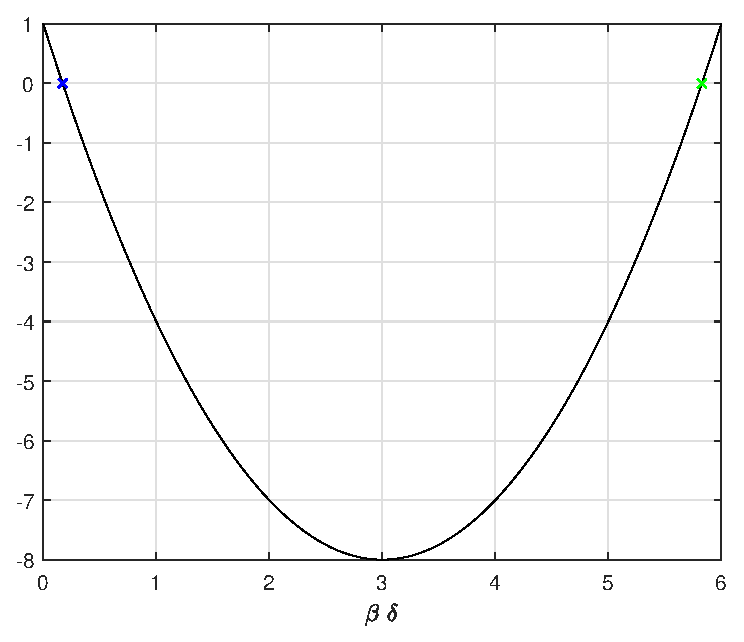
\includegraphics[width=0.7\linewidth]{bdregion.eps}
			\caption{A plot of the final condition with the positions of the zeros plotted}
			\label{fig:quadplot}
		\end{figure}



		\begin{figure}[tbh]
			\centering
			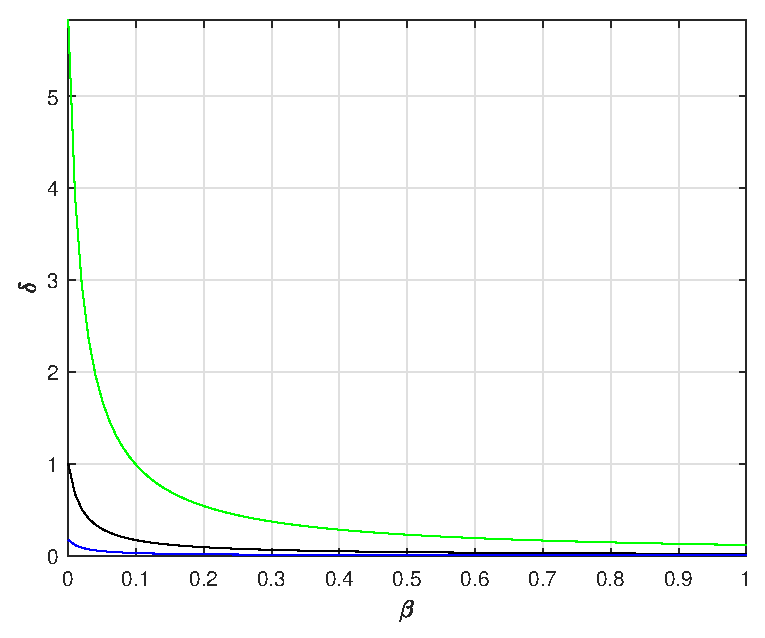
\includegraphics[width=0.7\linewidth]{betaVdelta.eps}
			\caption{A plot of the conditions together - colour coded to match the previous}
			\label{fig:condsplot}
		\end{figure}

		Figures~\ref{fig:quadplot} and~\ref{fig:condsplot} both show equalities for this to hold true. The colour coding is set to match the two plots together. 

		To satisfy the conditions the values of $\beta$ and $\delta$ must be above the green plot, as the blue plot is not in the valid region.




		
		\item From lectures $q=0$ is stable, and as $q^2\to\infty$ we have stability. 
		The $q$ with instability will be $q \in (q_1,q_2)$, where $(q_1,q_2)$ are the zeros of $h(q^2)$:
		\begin{align*}
			h(q^2) &= \delta q^4 - \gamma(\delta f_a + g_b)q ^2 + \gamma^2 \det M\\
			h(q^2) &= \delta q^4 - (\delta f_a + g_b)q ^2 + (f_a g_b - f_b g_a)\\
			&= \delta q^4 - (\delta \beta -1 ) q^2 +  \delta \beta\\
		\end{align*}
		\[
			q^2 = \frac{\beta \delta-1\pm\sqrt{\beta^2 \delta^2-4 \beta \delta^2-2 \beta \delta+1}}{2 \delta}
		\]
		So the unstable wavenumbers are 
		\[q^2 \in \left(\frac{\beta \delta-1-\sqrt{\beta^2 \delta^2-4 \beta \delta^2-2 \beta \delta+1}}{2 \delta}, \frac{\beta \delta-1+\sqrt{\beta^2 \delta^2-4 \beta \delta^2-2 \beta \delta+1}}{2 \delta}\right)\]


		\item By changing the rate of diffusion for $v$ to relate to $u$, at any instant, the rate of diffusion of $v$ could become quite small due to small $u$, and effectively bringing $\delta < 1$, hence ruining the possibility for the Turing instabilities to occur for small $u$. Near the steady state $(\beta^{-1},\beta^{-2})$ from before, the diffusion for $v$ would be approximately $\delta \beta^{-1}$.

	\end{enumerate}
	\item 
	\begin{enumerate}
		\item Information:
		\begin{itemize}
			\item nutrient diffuses, with diffusion coeff $D=1$
			\item Boundary conditions $c(x \geq L(t)) = c_\infty$.
			\item No flux at $x =0$, i.e. $\odd cx\pipe_{x=0} =0$
			\item $c<c_n$ causes necrotic cells
			\item necrotic cells do not consume nutrient
			\item necrotic cells decay at rate $\beta$.
			\item Diffusion of nutrient occurs faster than tumour growth
			\item Cell density is constant
		\end{itemize}
		Conservation of cells and nutrient give
		\begin{align*}
			\dd nt + \nabla \cdot(nv) &= f(c,\vec x,t)\\
			\dd ct + D\nabla^2 c &= \lambda n
		\end{align*}
		Given that the density of cells is constant$ D=1$, and prior to the necrotic region appearing, the reaction (proliferation) is $f \propto c$
		
		\begin{align*}
			\odd vx &= \gamma c\\
			\odd ct + \oddn cx2 &= \lambda\\
		\end{align*}
		Where $v$ is the velocity of cells, and $\gamma$ is the cell proliferation rate. For $0 < x < L(t)$, where $k$ is some constant consumption rate.

		The quasi-steady assumption gives $c = \frac{\lambda}{2} x^2 + bx + d$. $\odd cx\pipe_{x=0} = 0$ implies $b=0$.
		At $L$ we have $c(L) = c_\infty$ 
		\[c_\infty = -\frac{\lambda}{2} L^2 + d \implies d = c_\infty + \frac{\lambda}{2} L^2\]

		And we require that at $c(0)$ we are greater than $c_n$
		\begin{align*}
			c(0) = c_\infty + \frac{\lambda}{2} L^2 > c_n\\
			\implies L^2 < L^2_c = \frac{2(c_\infty - c_n)}{\lambda}
		\end{align*}

		Should have something like
		\[c = \frac12 \left(c_\infty - \lambda (L^2 - x^2)\right)\]
		%2 or 3 errors here
		Using this in the $v$ equation:
		\begin{align*}
			\odd vx &= \gamma c\\
			\odd vx &= \frac12\gamma \left(c_\infty - \lambda  x^2\right)\\
			\odd vx &= s\left(c_\infty - \lambda  x^2\right)\\
			v(x,t) &= sc_\infty x - \frac{\lambda s x^3}{3}\\
			v(L(t),t) &= sc_\infty L - \frac{\lambda s L^3}{3}
		\end{align*}

		The substitution $s = 2 \gamma$ implies that $s$ is twice the proliferation rate.
		Hence
		\[\odd Lt = s c_\infty L - \frac{\lambda s L^3}{3}\]

		\item The steady state $L=0$ is trivial:
		\begin{align*}
			\odd Lt &= s c_\infty L - \frac{\lambda s L^3}{3}\\
			\odd Lt &= 0 
		\end{align*}
		Stability:
		\begin{align*}
			\odd{}L\left(s c_\infty L - \frac{\lambda s L^3}{3}\right) &= s  c_\infty - \lambda s L^2\\
			&= s c_\infty
		\end{align*}
		Given $s, c_\infty > 0$ this is unstable.



		The $L = L_* \geq 0$ steady state:
		\begin{align*}
			\odd Lt &=s c_\infty L - \frac{\lambda s L^3}{3}\\
			0 &= s c_\infty - \frac{\lambda s L^2}{2}\\
			L^2 &= \frac{2 c_\infty }{\lambda}\\
			L &= \sqrt{\frac{2 c_\infty }{\lambda}}\\
		\end{align*}
		Ignoring the negative case since $L \geq 0$.
		Stability:
		\begin{align*}
			s  c_\infty - \lambda s L^2  &= s  c_\infty - \lambda s \frac{2 c_\infty }{\lambda}\\
			&= s c_\infty \left(1 - 2\right)\\
			&= - s c_\infty
		\end{align*}
		Given $s,c_\infty > 0 $ this is stable.


		%It cannot exist as the nutrient level at $x = 0$ 
		%show its impossible
		%not done yet
		\item 
		Inside the region $0 < x < L_n$, the (quasi steady) DEs are
		\[ \oddn cx2 = 0, \quad \odd vx = - \beta\]

		Solving gives
		\[v = - \beta r, \quad \]
		With $\lim_{x^- \to L_n}  c(L_n) =\lim_{x^+ \to L_n} = c(L_n) = c_n$ and $\lim_{x^- \to L_n} \odd c x = \lim _{x^+\to L_n}\odd cx$

		The length of the proliferating region $h = L - L_n$  as $L_n \to \infty$ and $L \to \infty$
		Look for the steady state as $t\to \infty$.
		The length of the necrotic region is obtained the same was as the tumour size 
		\[\odd L_n t = v(L_n)\]

		%not done yet
		\item 

		Need to get
		\[\odd Lt = s(L - L_n) \left(c_n + \frac \lambda 6 \left(L - L_n\right)^2 \right) - \beta L_n\]
		%not done yet
	\end{enumerate}
\end{enumerate}




\section*{Code}
\lstinputlisting{A3A4Code.m}
\includepdf[pages=1-]{A3_2019.pdf}
\includepdf[pages=1-]{A4_2019.pdf}


\end{document}

